\begin{figure*}[t]
\centering
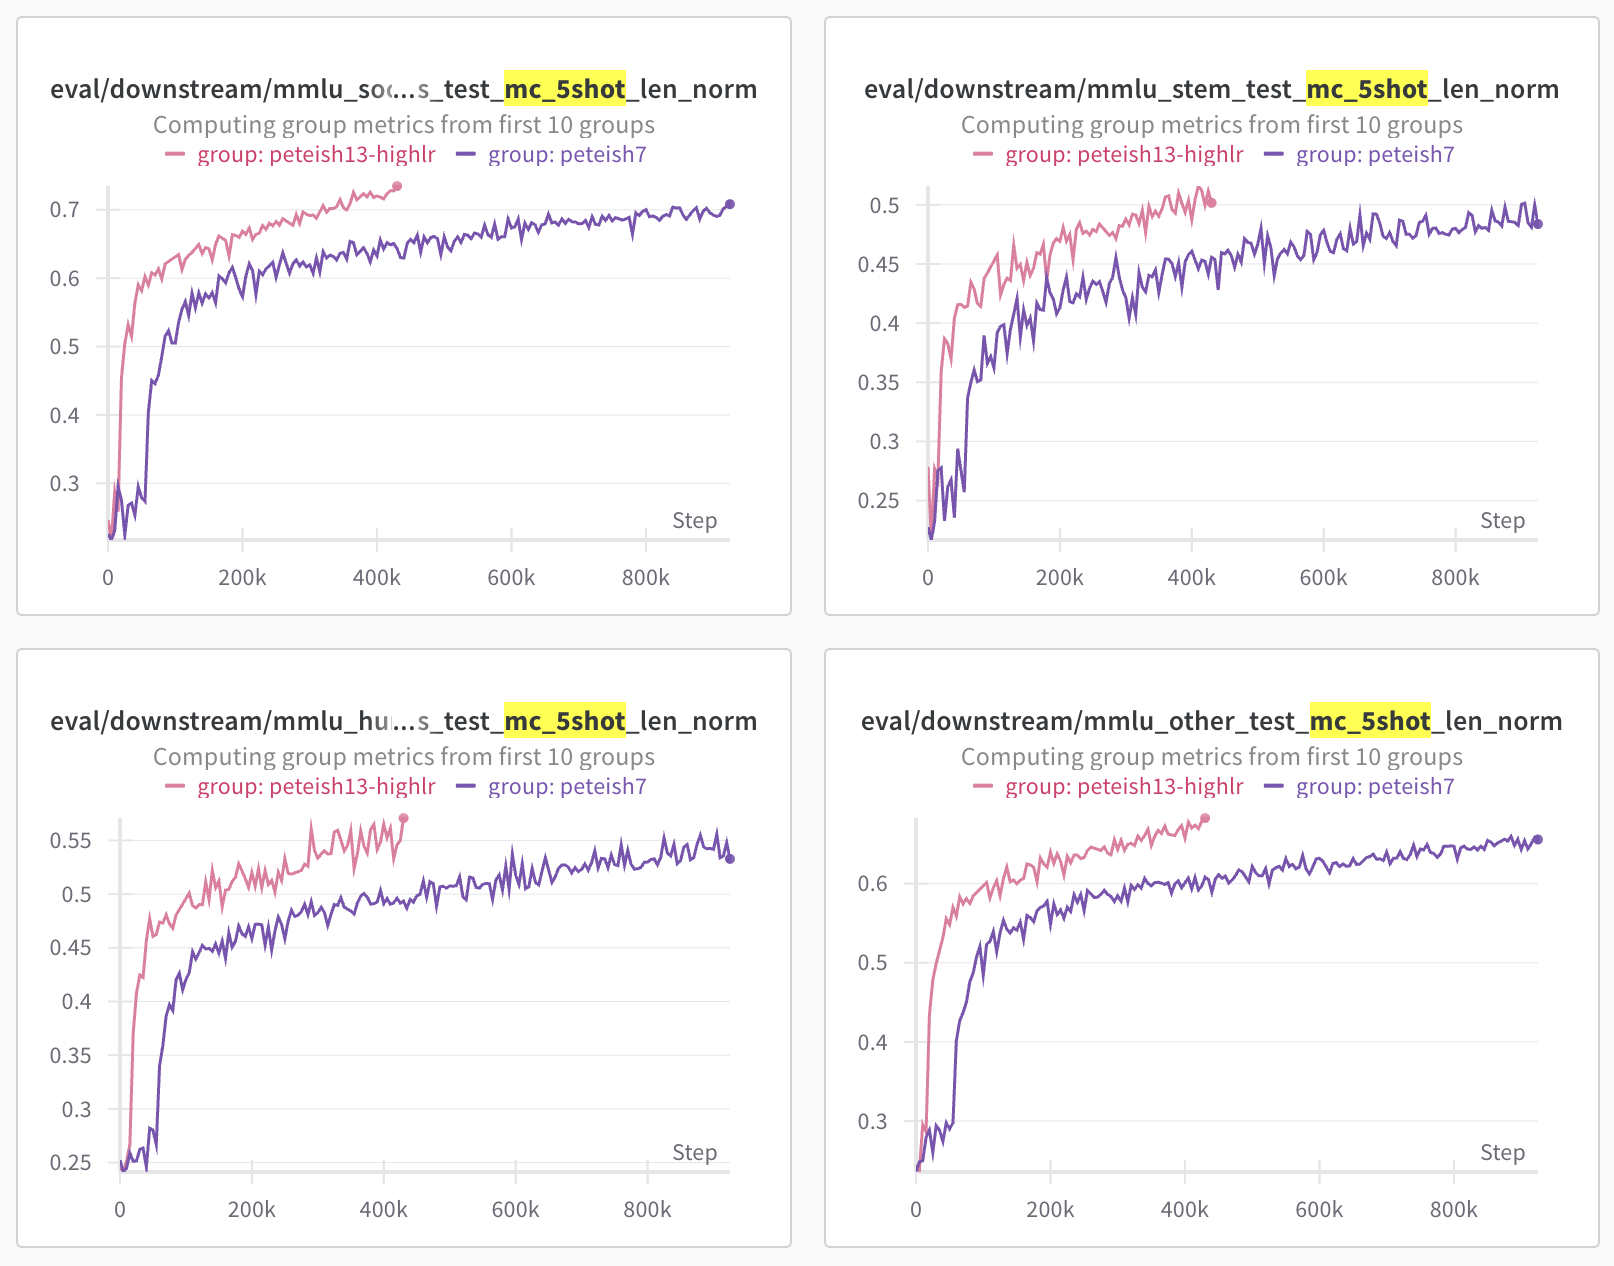
\includegraphics[width=0.39\linewidth]{images/mc_curves_mmlu.png}
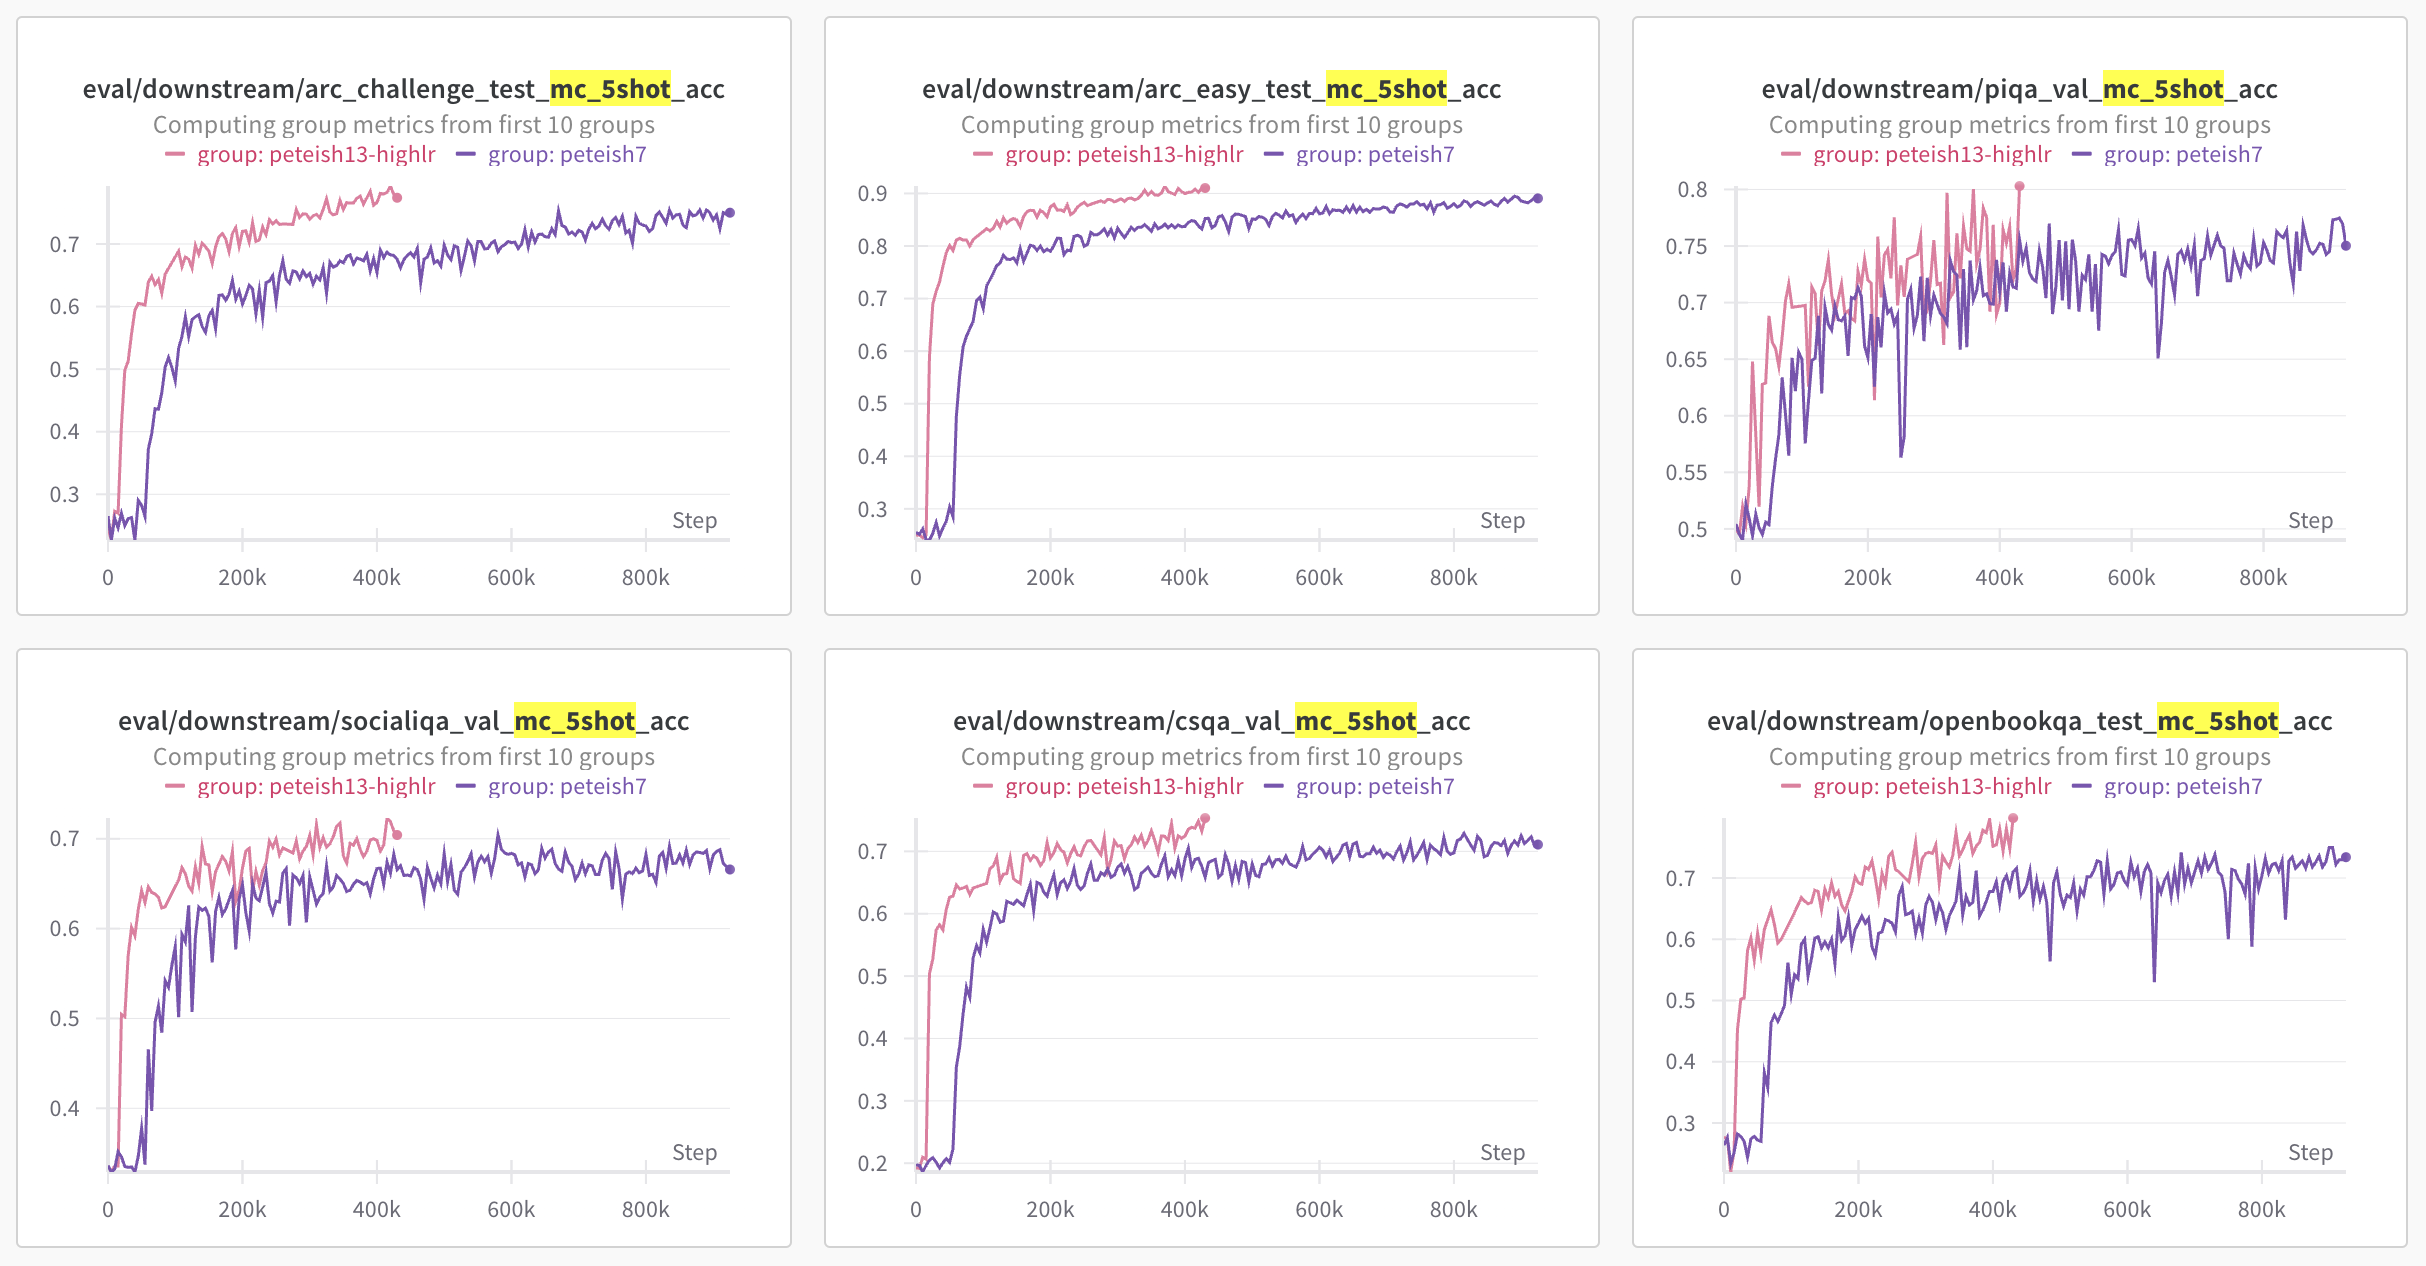
\includegraphics[width=0.59\linewidth]{images/mc_curves_core.png}
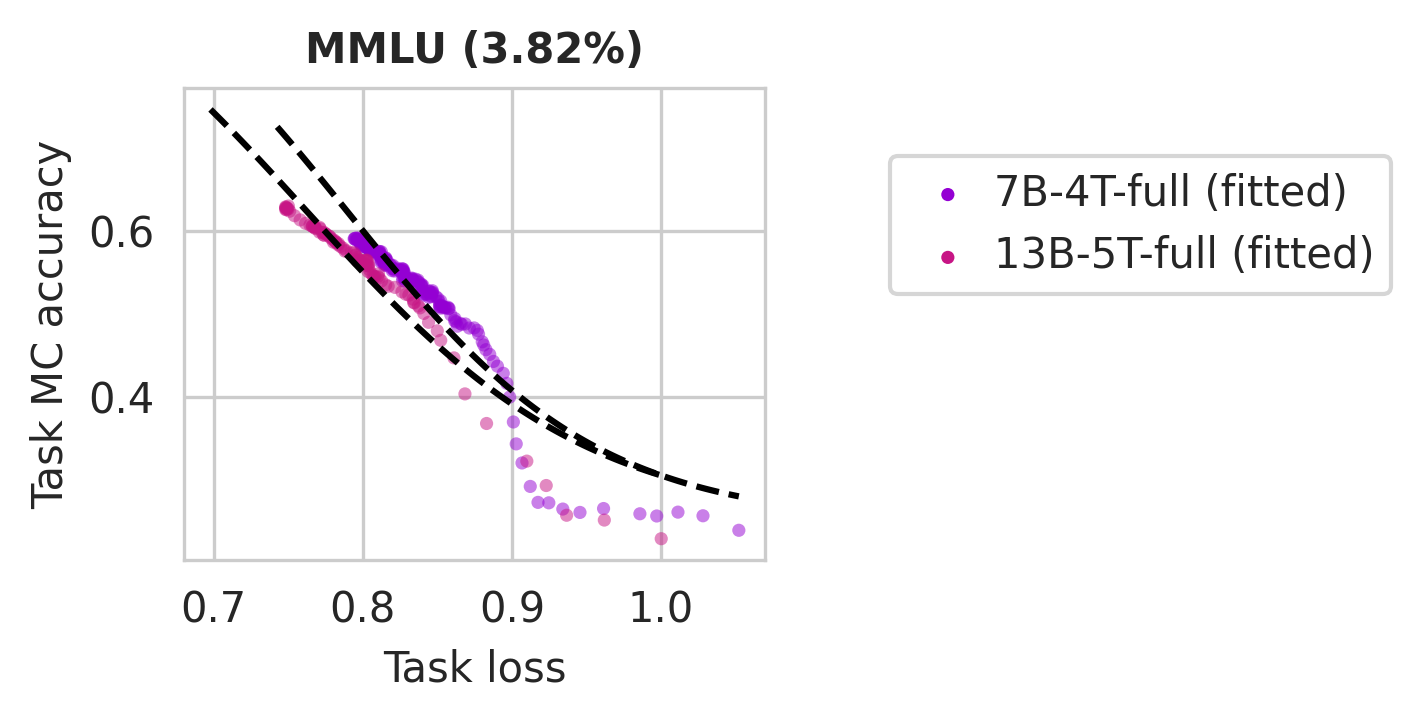
\includegraphics[width=0.49\linewidth]{images/step2_mc_mmlu_full.png}
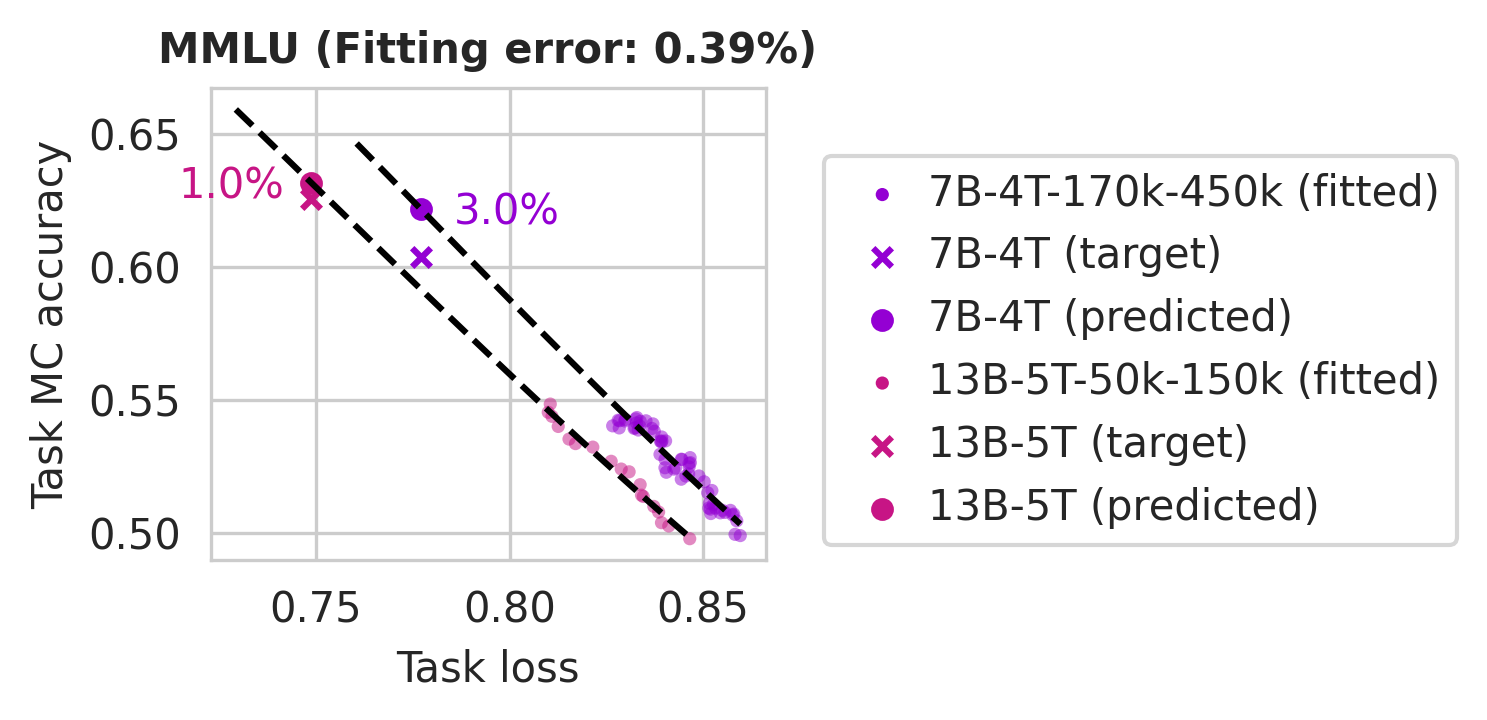
\includegraphics[width=0.49 \linewidth]{images/step2_mc_mmlu.png}
\caption{
    \textbf{Upper:} MC accuracy curves during training of 7B-4T and 13B-5T.
    \textbf{Lower left:} Task MC accuracy vs task loss, with data points from all intermediate checkpoints of 7B-4T and 13B-5T. A sigmoidal function cannot fit the data points.
    \textbf{Lower right:} Task MC accuracy vs task loss, where the sigmoidal function (\autoref{eqn:sigmoid}) is fitted on data points from the intermediate checkpoints between 170k--450k steps of 7B-4T, and between 50k--150k steps of 13B-5T.
}
\label{fig:step2_mc}
% \vspace{-16pt}
\end{figure*}